\documentclass[12pt]{article}

\usepackage{upgreek}

\usepackage{amsmath}

\usepackage{graphicx}
\graphicspath{ {imgs/} }

\usepackage{listings}

\usepackage{color}
 
\definecolor{codegreen}{rgb}{0,0.6,0}
\definecolor{codegray}{rgb}{0.5,0.5,0.5}
\definecolor{codepurple}{rgb}{0.58,0,0.82}
\definecolor{backcolour}{rgb}{0.95,0.95,0.92}
 
\lstdefinestyle{mystyle}{
    backgroundcolor=\color{backcolour},   
    commentstyle=\color{codegreen},
    keywordstyle=\color{magenta},
    numberstyle=\tiny\color{codegray},
    stringstyle=\color{codepurple},
    basicstyle=\footnotesize,
    breakatwhitespace=false,         
    breaklines=true,                 
    captionpos=b,                    
    keepspaces=true,                 
    numbers=left,                    
    numbersep=5pt,                  
    showspaces=false,                
    showstringspaces=false,
    showtabs=false,                  
    tabsize=2
}
 
\lstset{style=mystyle}

\usepackage{dsfont}

\usepackage{hyperref}

\usepackage[utf8]{inputenc}

\usepackage{mathtools}

\usepackage{textcomp}

\usepackage[english]{babel}

\usepackage{tikz}

\usepackage{tcolorbox}

\usepackage{amsthm,amssymb}

\setlength{\parindent}{0cm}

\renewcommand\qedsymbol{$\blacksquare$}

\usepackage{fancyhdr}
 
\pagestyle{fancy}
\fancyhf{}
\fancyhead[LE,RO]{Algorithm Design and Analysis -- Fall 2017}
\fancyhead[RE,LO]{Joshua Concon}
\fancyfoot[CE,CO]{\leftmark}
\fancyfoot[LE,RO]{\thepage}


\begin{document}

\title{CSCC73: Algorithm Design and Analysis\\ Lecture Notes}
\date{University of Toronto Scarborough -- Fall 2017}
\author{Joshua Concon}
\maketitle
Pre-reqs are CSCB63 and STAB52.
Instructor is Dr. Vassos Hadzilacos. He projects well so you can basically sit anywhere. If you find any problems in these notes, feel free to contact me at conconjoshua@gmail.com.

\tableofcontents

\pagebreak

\section{Wednesday, September 6, 2017}

\subsection{Greedy Algorithms}

All Greedy Algorithms are \underline{Optimization problems:} given input, compute output that
\begin{enumerate}
	\item{satisfies constraints}
	\item{optimizes (min or max) certain criteria}
\end{enumerate}

Solutions that satisfies constraints are called \textbf{feasible}.

\subsubsection{Interval Scheduling (KT 4.1)}

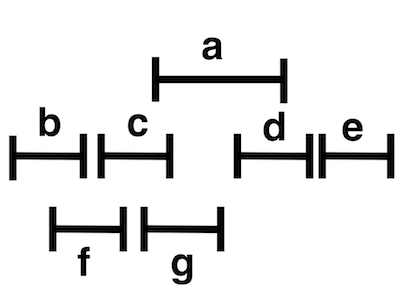
\includegraphics{interval1}\\
\\
\underline{Input:} Set of jobs $1,2,...,n$ where job $i$ has start time $s(i)$ and finish time $f(i) > s(i)$

\begin{tcolorbox}
	jobs $i,j$ conflict if each starts before the other finishes. i.e. if $s(i) < f(j)$ and $s(j) < f(i)$
\end{tcolorbox}

\underline{Feasible set of jobs:} A set where no two jobs conflict.\\
\\
\underline{Output:} A max cardinality feasible set (a max non-conflicting set of jobs) ('a set' rather than 'the set' as there may be more than 1 optimal sets.)\\
\\
\underline{e.g.} $\{ b,c,d,e \}, \{ b,g,d,e \}$ (from figure 1)\\
\\
\underline{Greedy "Schema":}\\
\begin{lstlisting}[language=Python]
sort jobs in some order
A := null
for each job i in sorted order do
	if i conflicts with no job in A then
		A := union of A and {i}
return A
\end{lstlisting}

We will make edits to this schema as we learn more about what sort order provides us with the most optimal set.

\subsubsection{Possible sort orders}

\begin{enumerate}
	\item{
	\textbf{sort by increasing start time}\\
	counterexample:\\
	\\
	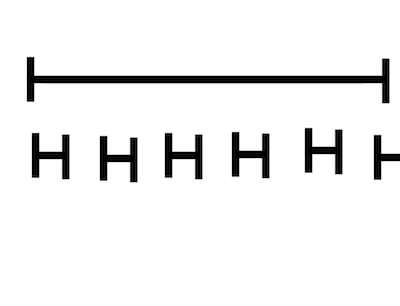
\includegraphics{interval2}\\
	\\
	As shown in the picture, the most optimal answer are the short intervals that come after the long interval has started, but the long interval is chosen first conflicting with the rest of the intervals.
	}
	\item{
	\textbf{sort by increasing duration length}\\
	counterexample:\\
	\\
	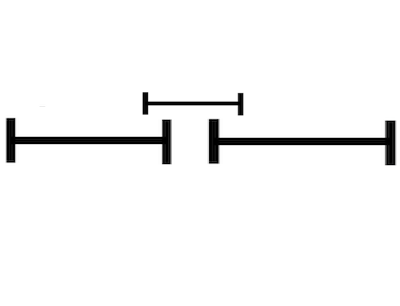
\includegraphics{interval3}\\
	\\
	The optimal answer in this picture is the two long intervals, but since there shorter interval is chosen and it conflicts with both of the long intervals, this sort does not work.
	}
	\item{
	\textbf{sort by increasing number of conflicts}\\
	counterexample:\\
	\\
	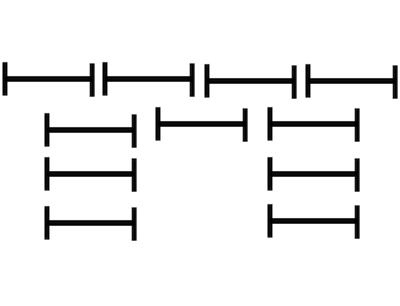
\includegraphics{interval4}\\
	\\
	In this case, the most optimal answer is all 4 of the top intervals. However, since it starts with the interval with the least amount of conflicts, it chooses an interval that conflicts with 2 of the 4 top intervals, which is the middle interval.
	}
	\item{
	\textbf{sort by increasing finish time}\\
	this increments $A$ using the smallest amount of time as possible, and this is also the correct sort for this algorithm.
	\\
	}
\end{enumerate}

\underline{Greedy "Schema" Revised:}\\
\begin{lstlisting}
sort jobs in increasing finish time
A := null
F := -infinity
for each job i in sorted order do
	if s(i) >= F then
		F := f(i)
		A := union of A and {i}
return A
\end{lstlisting}

\underline{Running Time:} $O(nlogn) + O(n) + O(1) = O(nlogn)$

\subsubsection{Proof of Correctness (optimality)}

Let $j_1, j_2, ... , j_k$ be jobs added to A in order considered

\paragraph{Claim 1:} A is feasible, proof trivial (just use sort by increasing finish time in the scheme, nothing in A should conflict by the algorithm).\\
\\
Let $j_1^*, j_2^*, ... , j_m^*$ be jobs in some optimal $A^*$ (in left to right order)
\paragraph{Claim 2:} $f(j_t) \leq f(j_t^*), \forall t, 1 \leq t \leq k$ (greedy algorithm stays ahead)

\begin{proof}
(proof of Claim 2)\\
Use induction.\\
\\
\underline{Basis:} $t=1$, algorithm adds interval with earliest finish time to $A$, so this holds.\\
\\
\underline{Induction Step:} For contradiction, assume $f(j_{t+1}) > f(j_{t+1}^*)$. This is immpossible because $f(j_t) \leq f(j^*_t)$ and the Induction Hypothesis Algorithm has not considered $j^*_{t+1}$ yet and will consider $j^*_{t+1}$ before $j_{t+1}$ and will add $j^*_{t+1}$ to $A$ instead of $j_{t+1}$.\\
\\
\underline{Induction Hypothesis:} $f(j_t) \leq f(j^*_{t})$\\
\\
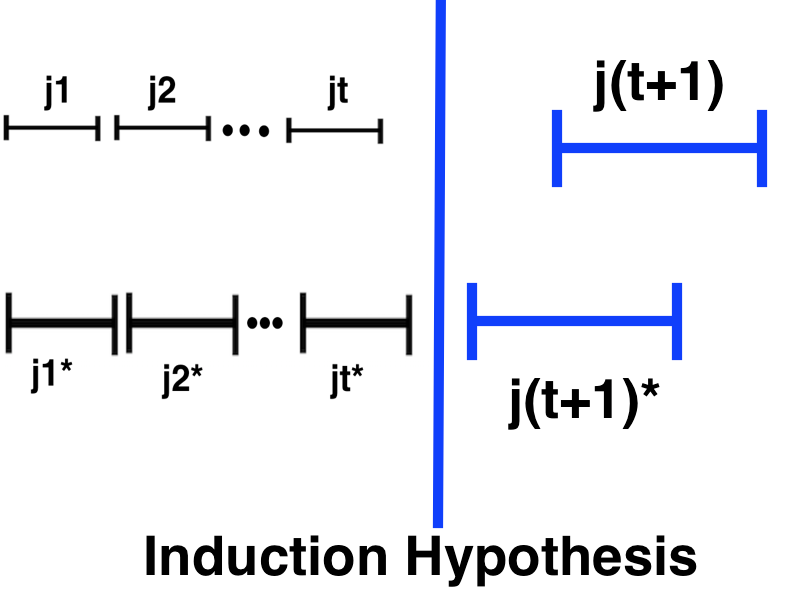
\includegraphics{interval5}\\
\\
Assume for contradiction: $f(j_{t+1}) > f(j_{t+1}^*)$.\\
\\
We have... 
\begin{align*}
	f(j_t) &\leq f(j_t^*)\:\:\:\text{by Induction Hypothesis}\\
	&\leq s(j_{t+1}^*)\:\:\:\text{Because $A^*$ is feasible and jobs are labelled left to right}\\
	&< f(j_{t+1}^*)\:\:\:\text{Finish time is strictly greater than start time}
\end{align*}

Immediately after the algorithm adds job $j_t$ to $A$, job $j^*_{t+1}$:
\begin{itemize}
	\item{has not been considered $(f(j_t) < f(j^*_{t+1})$}
	\item{$j^*_{t+1}$ does not conflict with jobs in $A$ as $f(j_t) \leq f(j^*_t) \leq s(j_{t+1}^*)$}
	\item{$j^*_{t+1}$ has priority over $j_{t+1}$ (by assumption, $f(j_{t+1}) > f(j^*_{t+1})$)}
\end{itemize}

Therefore $j_{t+1}$ is not the next job added to $A$ by the algorithm, therefore there is a contradiction. So Claim 2 must be true.

\end{proof}

\paragraph{Claim 3:} $k=m$

\begin{proof}(Proof of Claim 3)\\

Clearly $k\leq m$, since m is optimal.\\
Assume for contradiction that $k < m$\\
\\
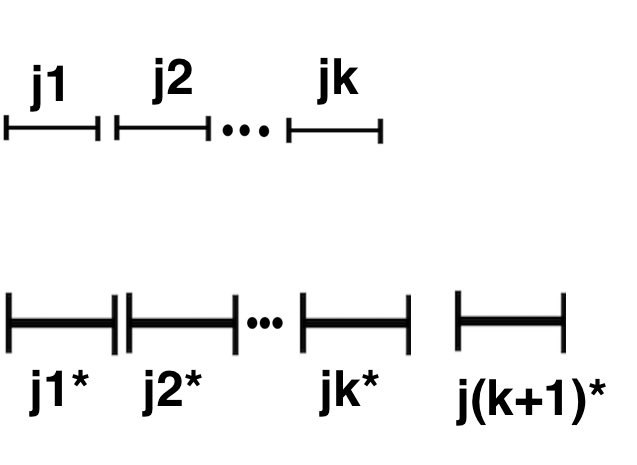
\includegraphics{interval6}\\
\\
But then $j^*_{k+1}$ should also be in $A$, but it's not in $A$. Therefore it doesn't exist.\\
\\
Therefore $k=m$
\end{proof}

\underline{Alternative Approach ("promising set"):}\\
For each iteration $i$ in a Greedy Algorithm, there exists an optimal set $A^*$ such that $A_i \subseteq A^*$\\

\underline{Generalization of Interval Scheduling:}\\
Interval Scheduling can be generalized to cover different problems, such as Weighted Intervals, finding the minimum amount of concurrent machine to perform all intervals.

\newpage

\section{Monday, September 11, 2017}

\subsection{Min-Max Lateness (KT 4.1)}

\underline{Input:}
\begin{itemize}
	\item{release time $r$ (earliest time to start all jobs)}
	\item{$n$ jobs $1,2,...,n$}
	\item{for each job $i$}
	\begin{itemize}
		\item{length $t(i) \geq 0$}
		\item{deadline $d(i)$}
	\end{itemize}
	\item{can only do jobs one at a time}
\end{itemize}

We want to minimize the maximum lateness of any job.\\
\\
\underline{Schedule:} $S$ specifies start time of each job $i$. $(s(i) \geq r)$\\
\\
end time of $i = s(i) + t(i)$, such that $[ s(i), s(i)+t(i) ]$ and $[ s(j), s(j)+t(j) ]$ do not overlap for all jobs $i,j$ where $i \neq j$\\
\\
\underline{Output:} Find an $S$ that minimizes the max lateness of any job.\\

\textbf{Example:}

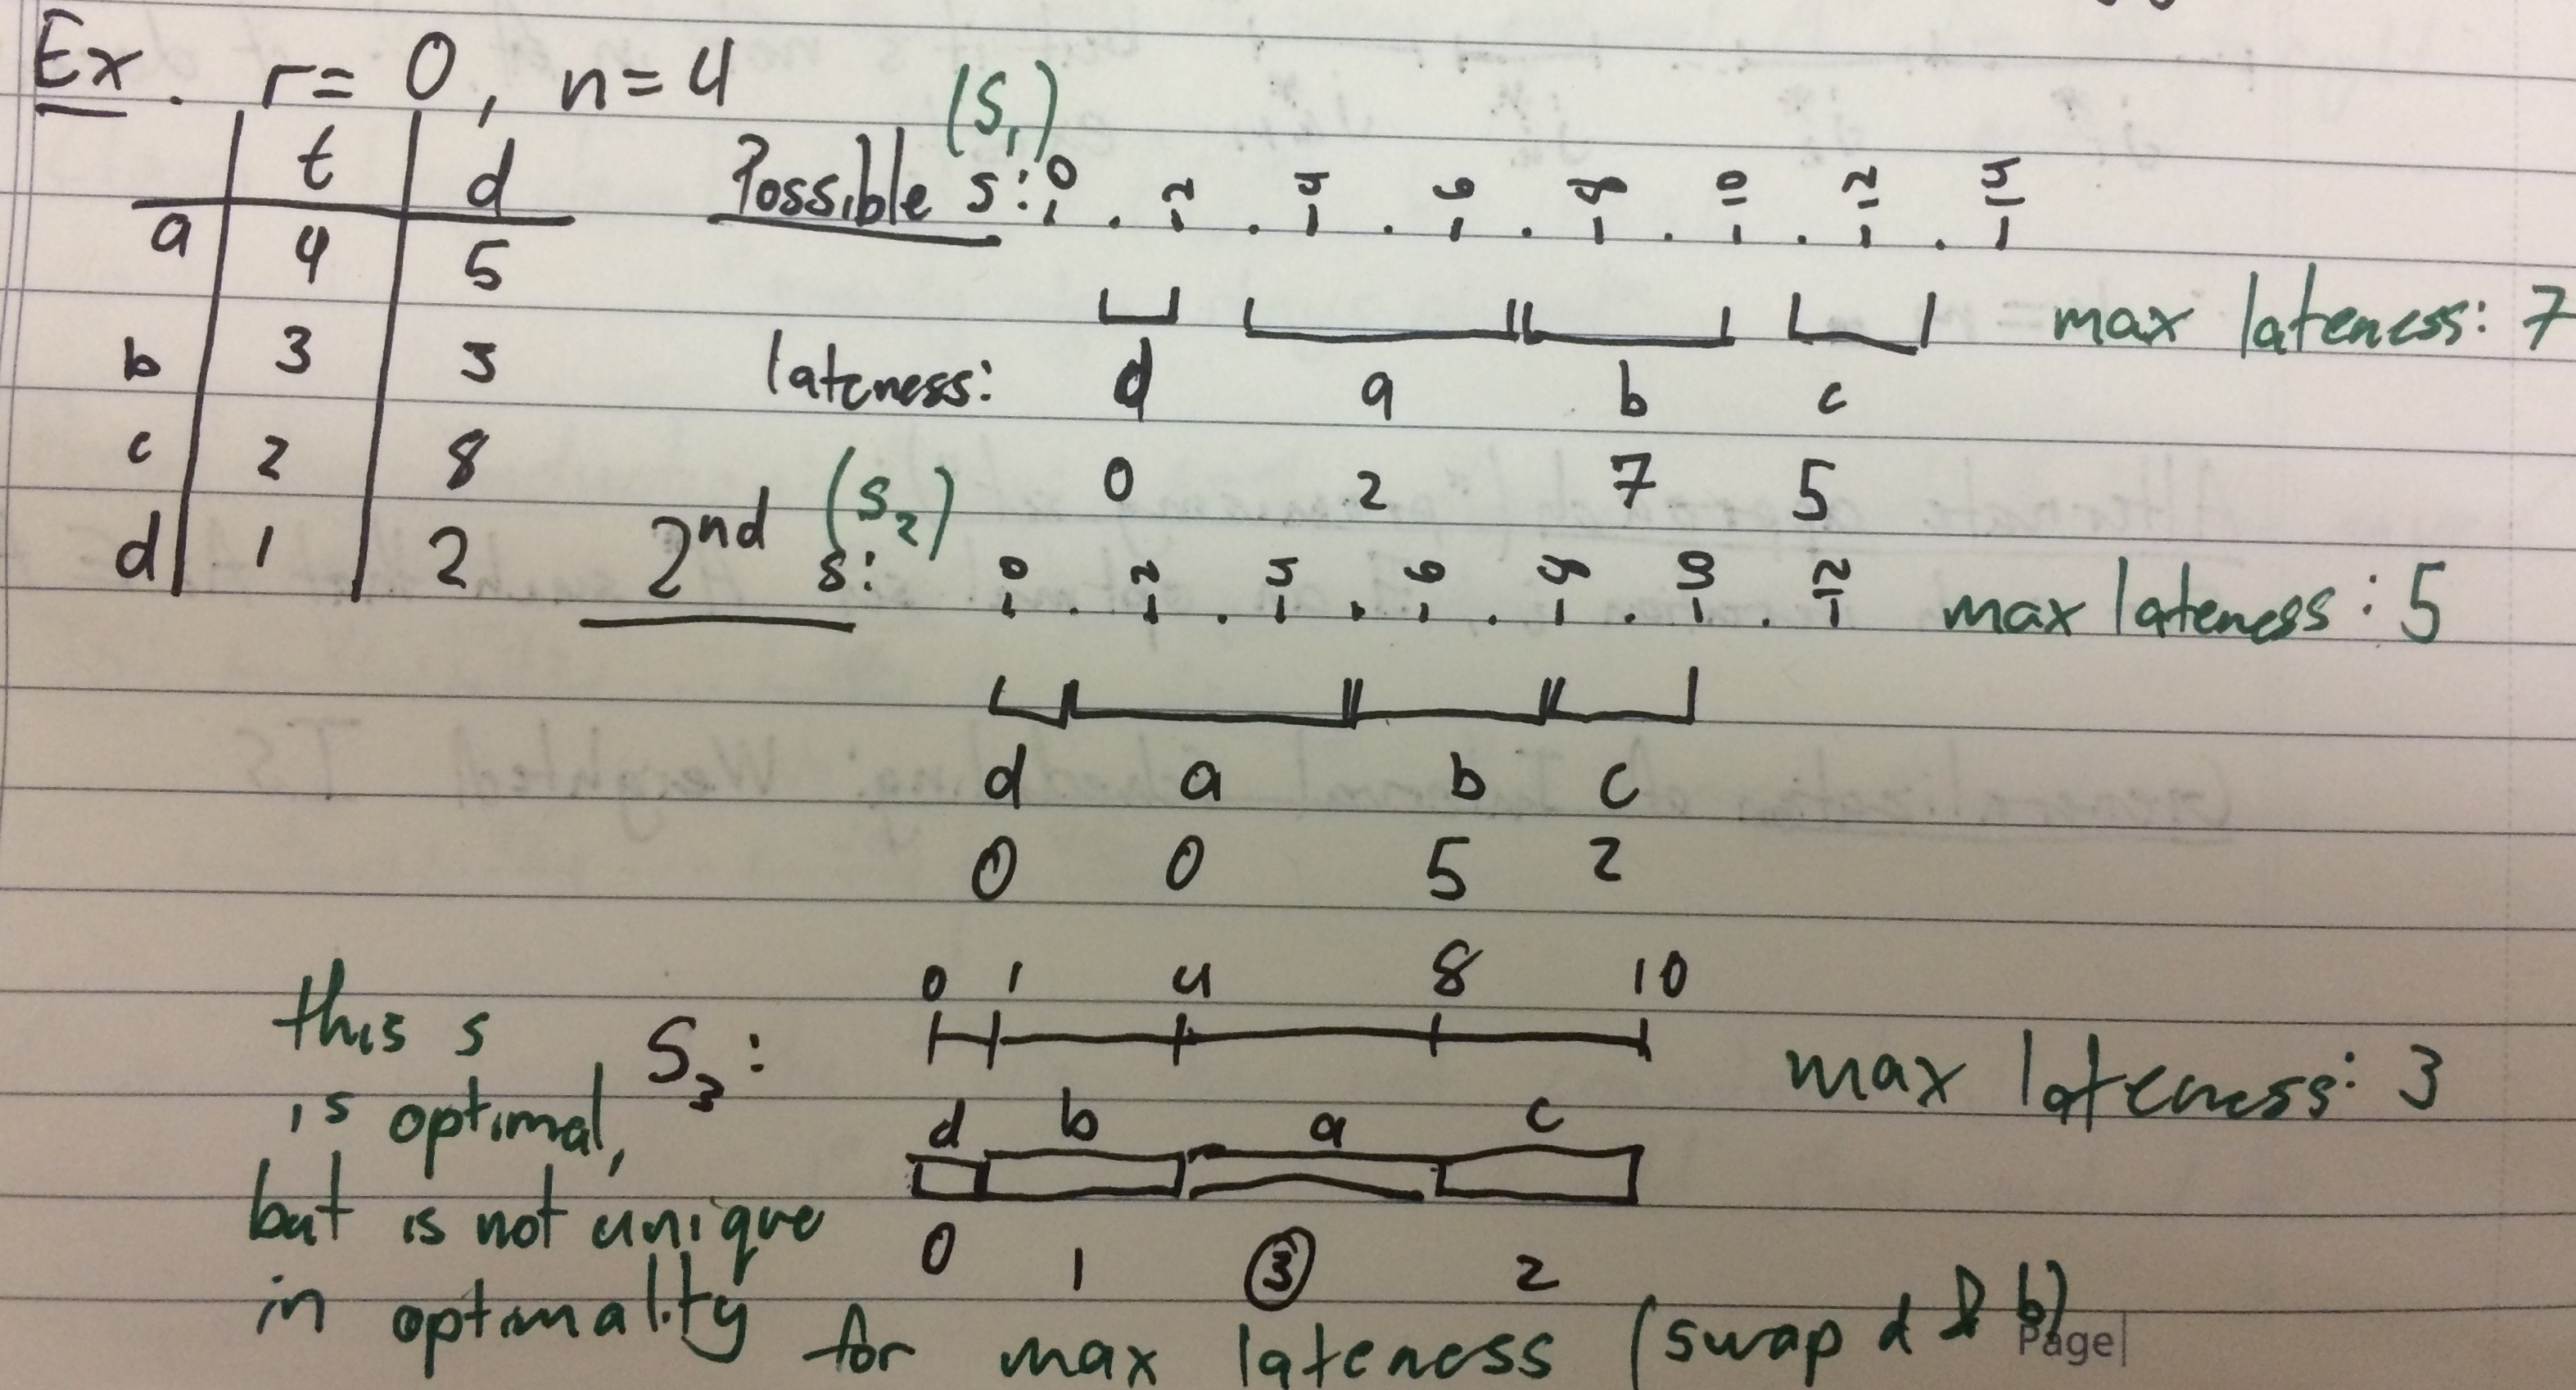
\includegraphics[scale=0.15]{minmax1}

This $S$ is optimal, but is not unique in optimality for the smallest max lateness (you can get another optimal solution by swapping $d$ and $b$)\\

\underline{Algorithm (Earliest Deadline First):}

\begin{lstlisting}[language=Python]
ALGO:
	Sort jobs by increasing deadline
	Let d[1,..,n] be deadlines (in sorted order)
	Let t[1,...,n] be durations of corresponding jobs
	F := r # max finish time of all jobs schedules so far
	for i:= 1 to n do
		gs(i) := F
		F := gs(i) +t (i)
	return gs
\end{lstlisting}

\underline{Running Time:} $\Theta (nlogn)$\\
\\
\begin{tcolorbox}[title=Inversion]
	An \textbf{inversion} in schedule $S$ is a pair of jobs $i,j$ such that $s(i) < s(j)$ but $d(i) > d(j)$\\
	\\
	\underline{i.e.}\\
	 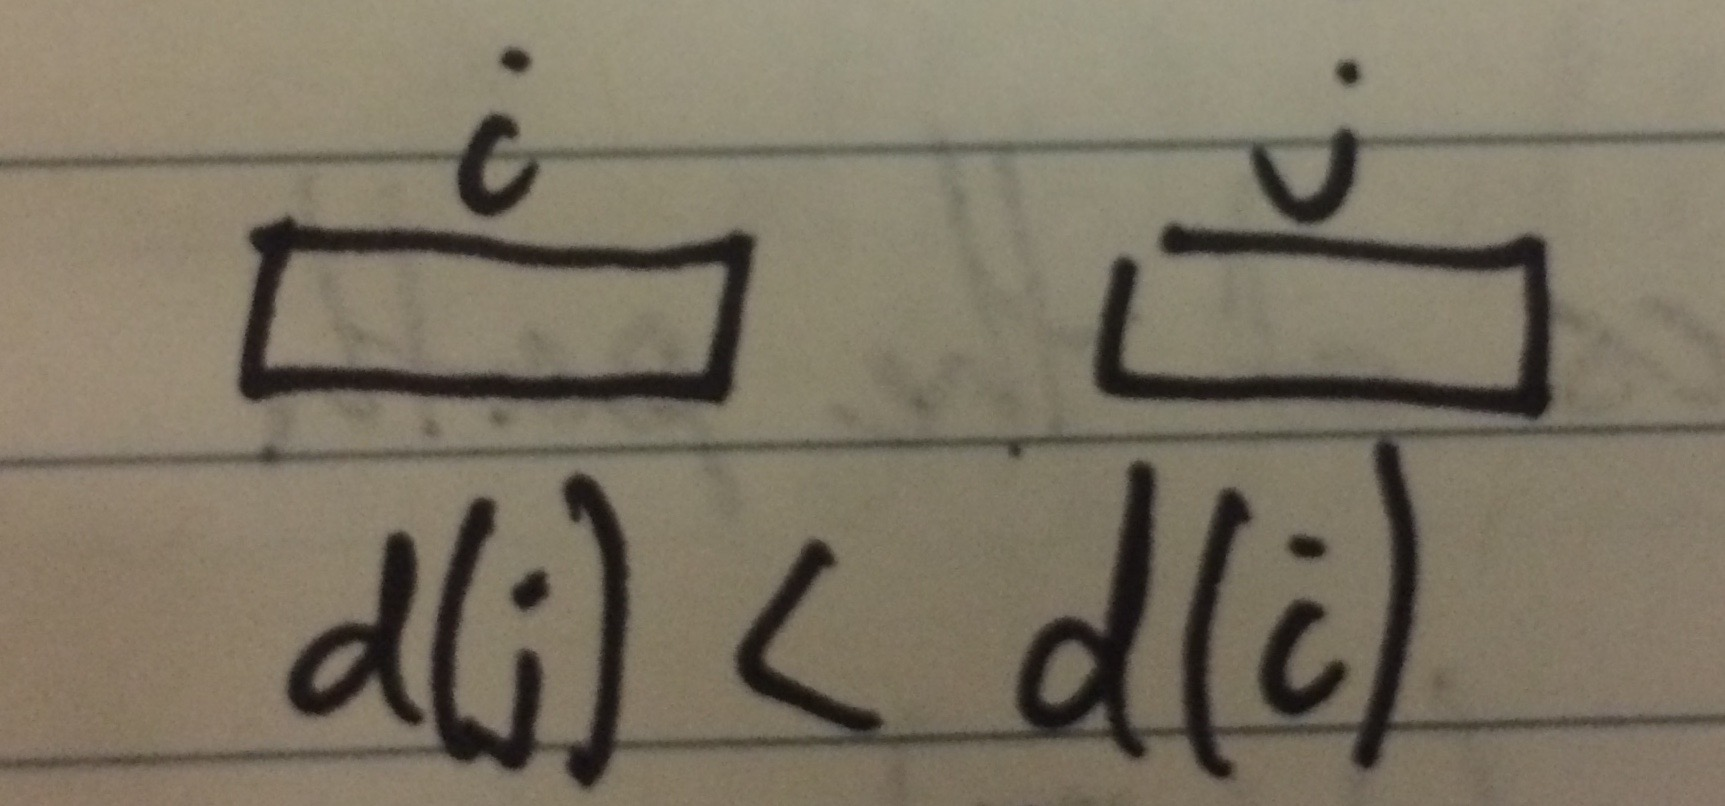
\includegraphics[scale=0.1]{minmax2}
\end{tcolorbox}

This algorithm has no gaps and no inversions, which both properties ensures optimality.\\
\\

\begin{tcolorbox}[title=Theorem]
	Any schedule with no gaps and no inversions is optimal
\end{tcolorbox}

\underline{Observation 1:} There is an optimal schedule with no gaps\\
\\
\underline{Observation 2:} All schedules with no gaps or inversions have the same max lateness\\
\\
Given $S$ with no gaps and at least 1 inversion, there exists a pair of jobs $i,j$ that have an inversion and are consecutive in s.\\
\\
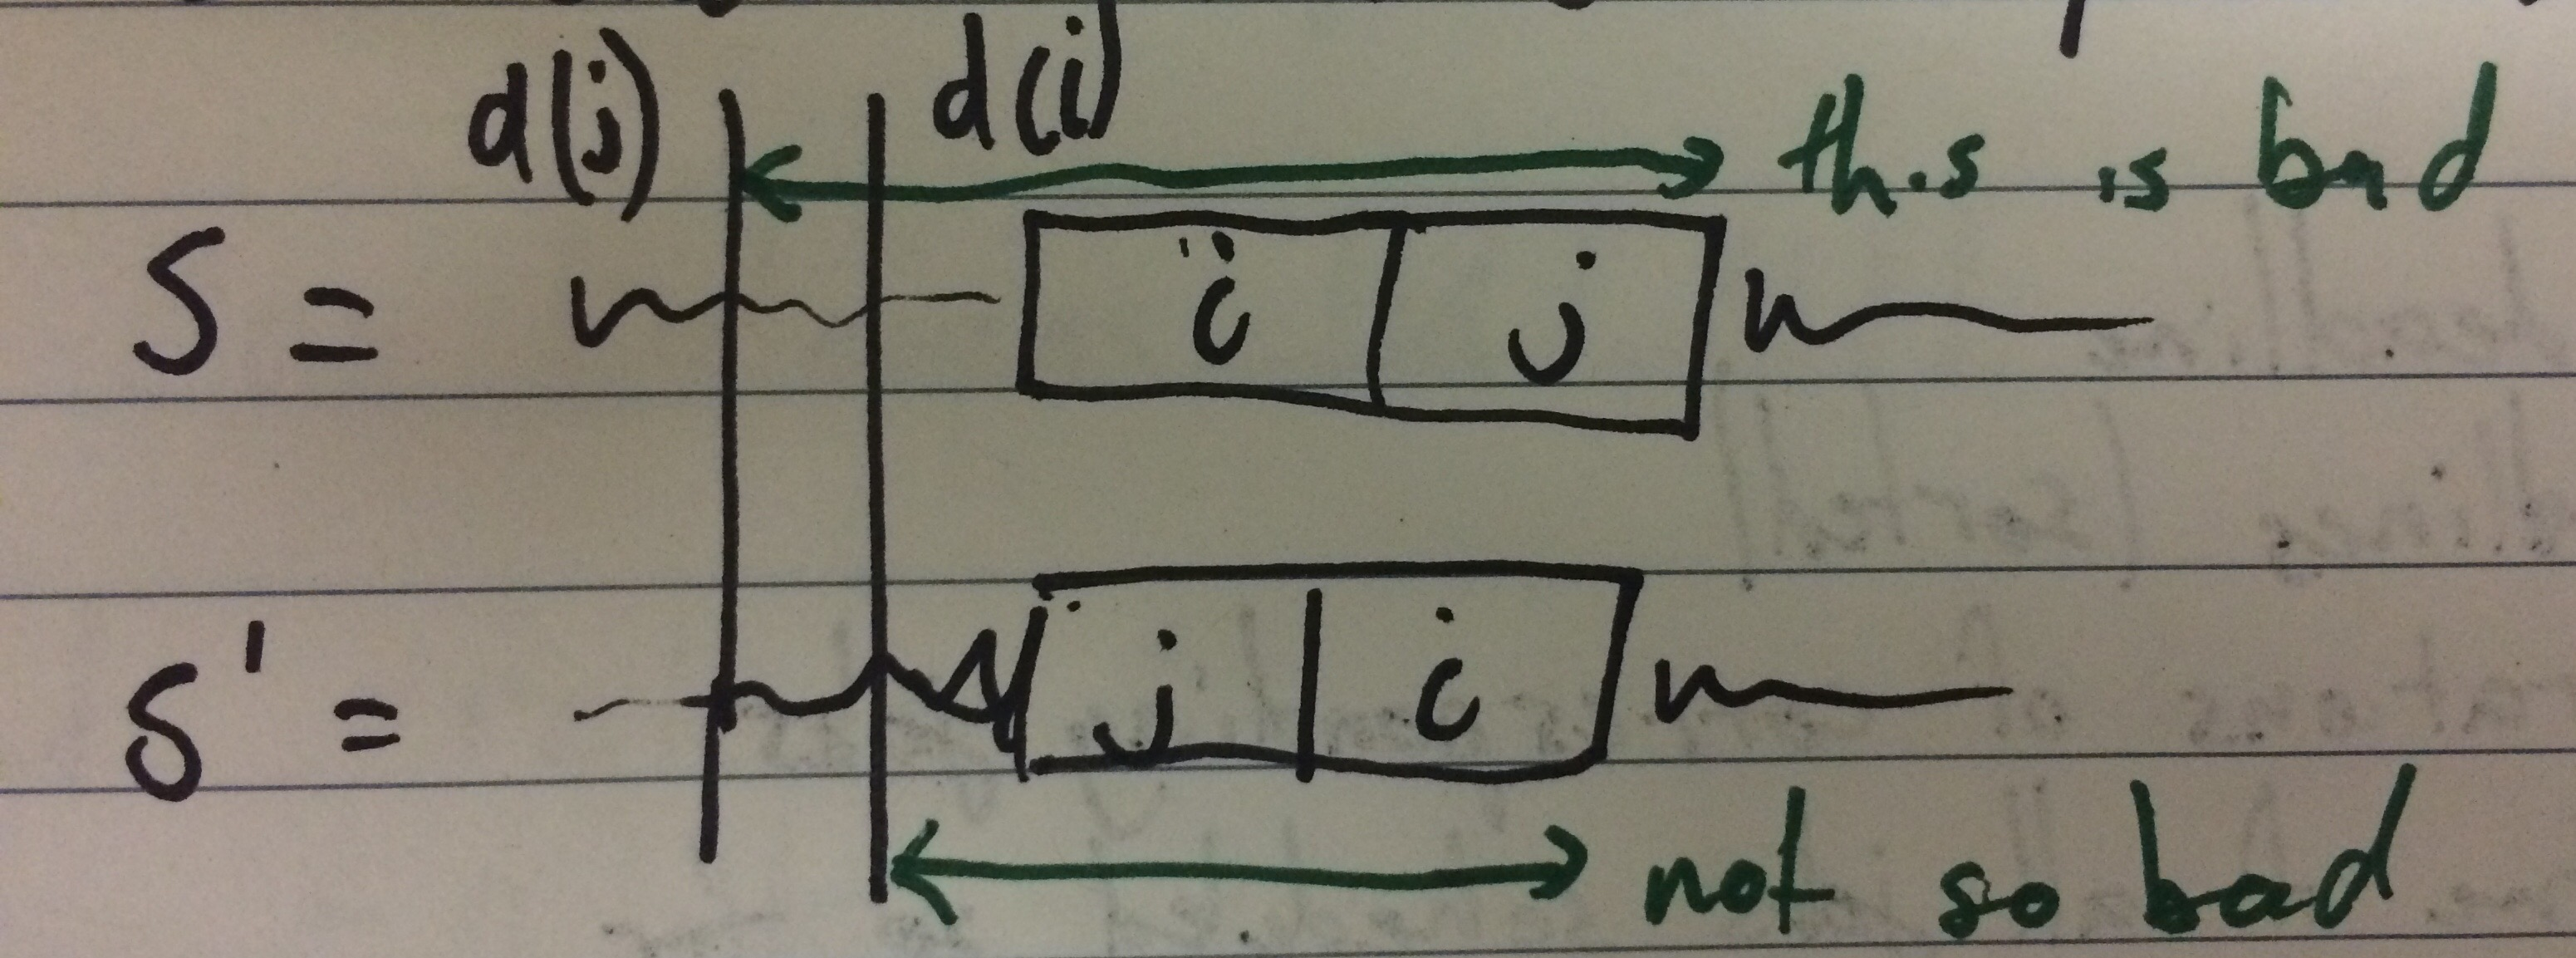
\includegraphics[scale=0.11]{minmax4}
\\
\\
Let $S'$ be a schedule like $S$ except $i,j$ are swapped.\\
\\
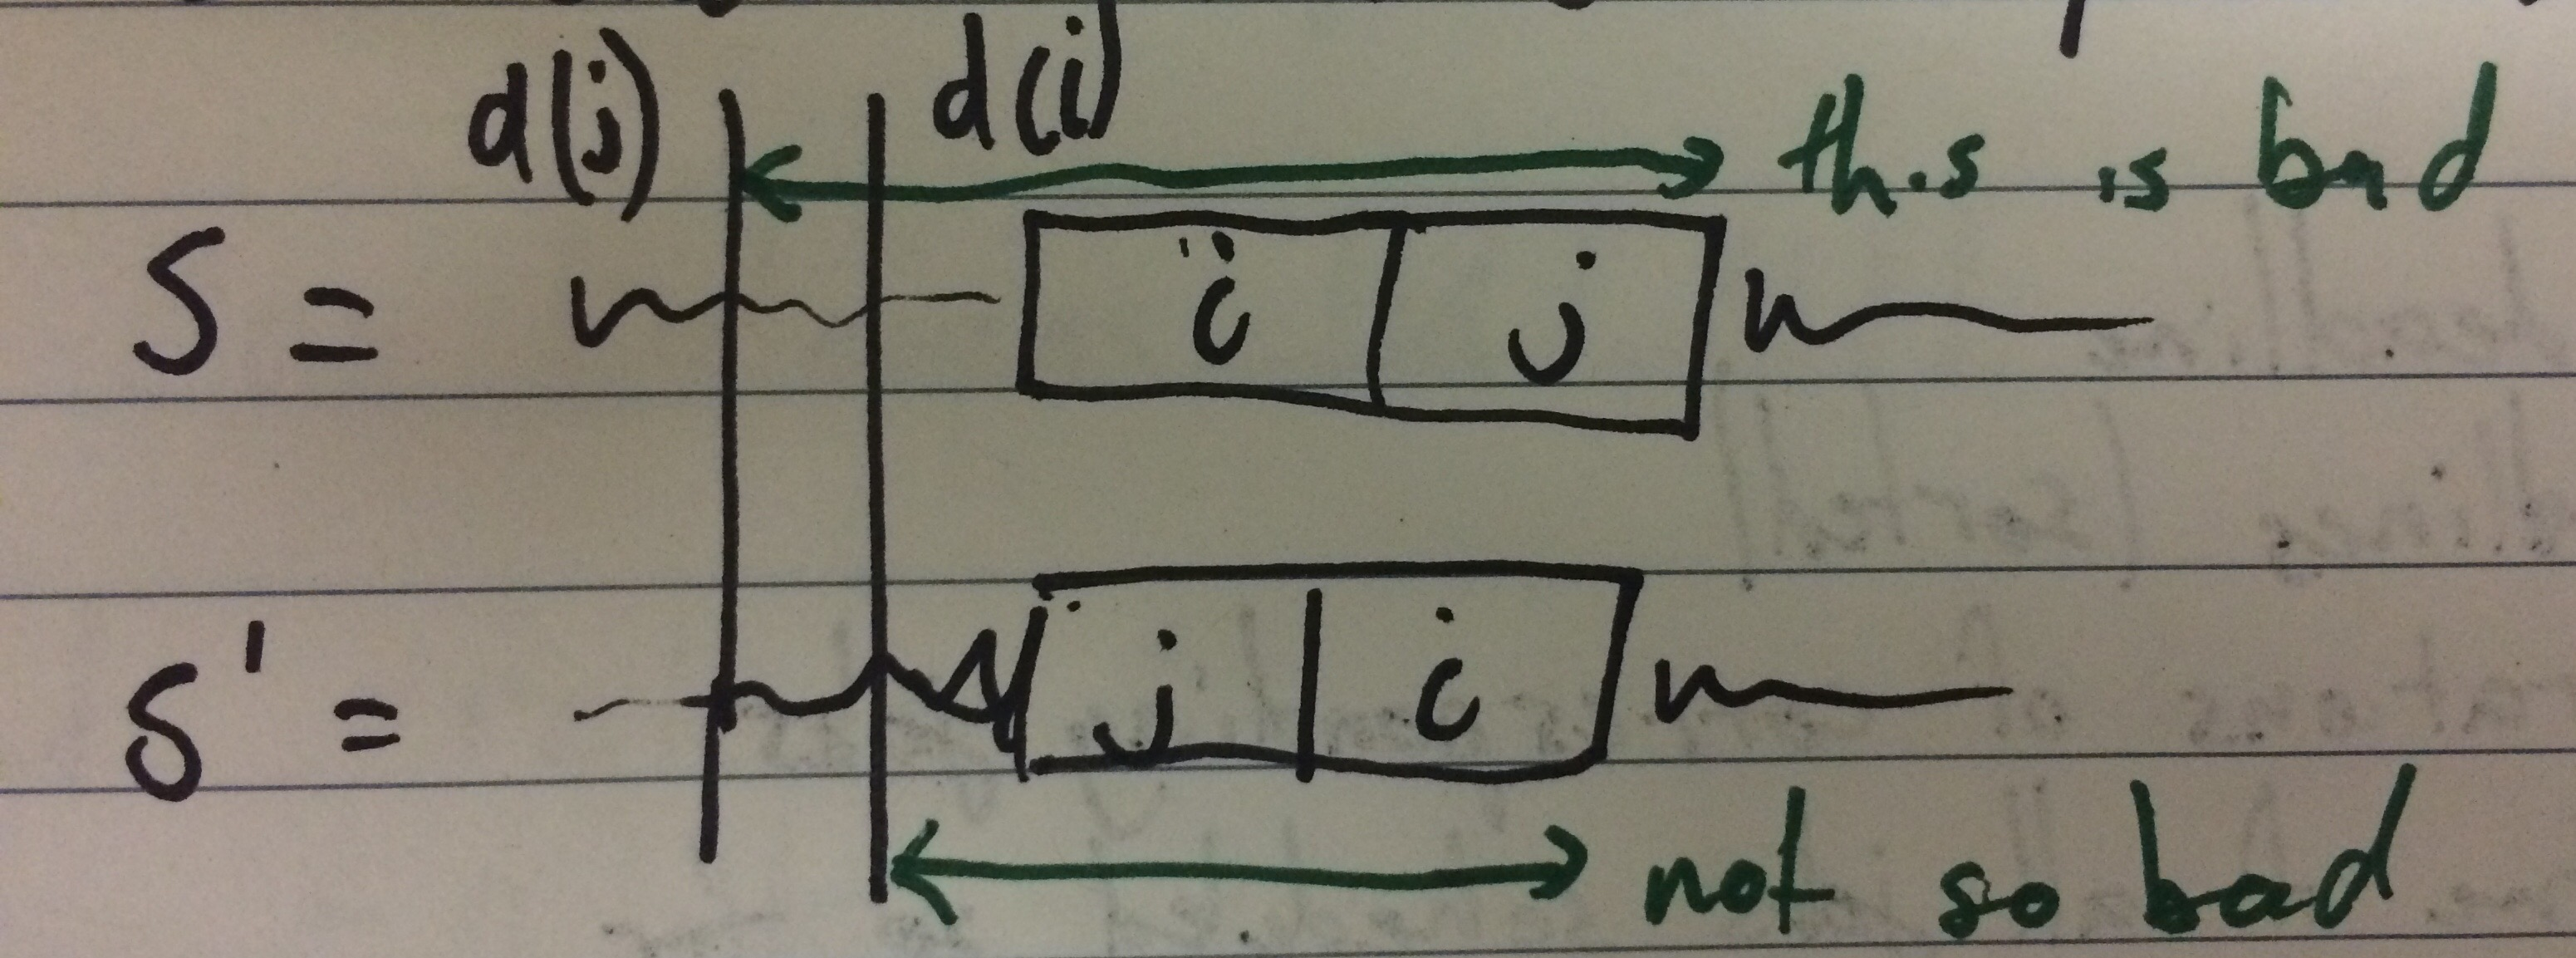
\includegraphics[scale=0.11]{minmax4}
\\
\\
\begin{itemize}
	\item{All jobs that are not $i,j$ have the same lateness in $S$ as in $S'$}
	\item{Lateness of $j$ in $S'$ does not increase}
	\item{Lateness of $i$ in $S'$ may increase though, but less than lateness of $j$ in $S$}
\end{itemize}
This implies that the max lateness in $S'$ $\leq$ max lateness in $S$.

\newpage

\section{Wednesday, September 13, 2017}

\subsection{Dijkstra's Shortest Path Algorithm (KT 4.4, DPV 4.4)}

$wt(P) = $ sum of the weights of edges of the path $P$\\
\\
\underline{Input:} 
\begin{itemize}
	\item{Weighted (di)graph $(G=(V,E))$}
	\item{source node $s\in V$}
	\item{weight of edges $wt(u,v) \geq 0, \forall (u,v) \in E$}
\end{itemize}

\underline{Output:} $\forall v \in V$
\begin{itemize}
	\item{$\delta (v) = $ minimum weight of $s \rightarrow v$ path}
	\item{$p(v) = $ predecessor of $v$ on a shortest $s \rightarrow v$ path}
\end{itemize}

We must maintain a set of nodes $R$, and $\forall u\in V, d(u)$

\underline{Intervals:}
\begin{enumerate}
	\item{$\forall u\in V, d(u) = $ minimum weight of any $s \rightarrow u$ path in which all nodes that are not $u$ are in $R$ ("$R$ - path")\\
	\\
	\underline{Visualization:}\\
	\\
	(insert pic here)
	\\
	\\
	or $d(u) = \infty$, if no such path exists}
	\item{$\forall u \in R, \forall u' \not\in R, d(u) \leq d(u')$}
\end{enumerate}

\underline{Note:}
\begin{itemize}
	\item{$\forall u, d(u) \geq \delta (u)$}
	\item{$\forall u \in R, d(u) = \delta (u)$}
\end{itemize}

\subsection{Algorithm}

\begin{lstlisting}[language=Python]
ALGO:
	R := {s}
	d(s) := 0
	p(s) := NULL
	for each node u != s do
		if (s,u) in E then
			d(u) := wt(s,u)
			p(u) := s
		else
			d(u) := infinity
			P(u) := NULL
	while R != V do
		let v be node not in R such that d(v) is min
		R := UNION(R,v)
		for each node u such that (v,u) in E do
			if d(u) > d(v) + wt(v,u)
				d(u) := d(v) + wt(v,u)
				p(u) := v
\end{lstlisting}

\underline{Visualization:}\\
\\
(insert pic here)

\subsection{Running Time}

($n = |V|, m = |E|$)

\begin{enumerate}
	\item{ \underline{Native Implementation:} $O(n) + O(n)O(n) = O(n^2)$\\
	\\
	The first $O(n)$ from the left is the running time for the initialization of all nodes before the while loop begins, the second $O(n)$ refers to how many times the while loop runs, and the last $O(n)$ refers to how long each loop takes. This results in a running time of $O(n^2)$}
	\item{ \underline{"Sophisticated" Implementation:}\\ $O(n) + O(n) + O(nlogn) + O(mlogn) = O((n+m)logn)$ or $O(mlogn)$ if it is assumed that there are no unreachable nodes from $s$}\\
	\\
	The first $O(n)$ refers to the initialization of all nodes before the while loop begins, the second $O(n)$ refers to the execution of BUILDHEAP on the nodes, the $O(nlogn)$ refers to the $O(n)$ EXTRACTMIN operations from this heap, and $O(mlogn)$ refers to all the change key operations for this heap.
\end{enumerate}

$O(n^2)$ vs. $O(mlogn)$, worst case $m = n^2$ (all nodes are connected to a linear amount of nodes).\\
\\
if $G$ is "dense" (i.e. $m = \Theta (n^2)$) then naive is faster\\
if $G$ is "sparse" then it's the opposite

\underline{Why non-negative weights for the edges?}\\
\\
(insert picture here)
\\
\\
With $s = A$, the fastest route to $C$ from $A$ is $A \rightarrow B \rightarrow C$ which is wrong.

\subsection{Correctness}

$R_i, d_i = $ values of $R,d$ at the end of $i$th iteration.

\paragraph{Claim 1:} If invariants $(1)$ and $(2)$ hold. $\forall u \in R_{i+1}, d_i (u) = \delta (u)$\\
(\underline{Note:} $R_{i+1} = R_i \cup \{ v \}$)

\begin{proof}
	(Proof of Claim 1:)\\
	Let $u \in R_i \cup \{ v \}$ and $P$ be a minimum weight $s \rightarrow u$ path.\\
	\\
	If $P$ is on $R_i$-path, then done by invariant (1)
	If $P$ is not on $R_i$-path...\\
	\\
	(insert picture)
	\\
	\\
	Note how $u' \in R_i$, and $u \in R_{i+1}$
	\begin{align*}
		\delta (u) &= weight(P)\\
		&\geq weight(P') \:\:\:\text{since $wt \geq 0$}\\
		&\geq d_i (u') \:\:\:\text{by invariant 1, since $P'$ is an $s \rightarrow u'$ is an $R_i$ - path}\\
		&\geq d_i (u) \:\:\:\text{if $u\in R_i$ by invariant 2, $u=v$ by choice of $v$}\\
		&\geq \delta (u) \:\:\:\text{[since $\forall u, d(u) \geq \delta (u)$]}
	\end{align*}
	
	and this implies that $d_i (u) = \delta (u)$

\end{proof}

Why if invariants (1) and (2) hold after the $i$th iteration, invariant (1) holds after $(i+1)$st iteration for nodes $u \not\in R_{i+1}$\\
\\
Let $P$ be minimum-weight $s\rightarrow u$ $R_{i+1}$-path with the fewest occurrences of the new node $v$.\\
\\
\underline{Case 1: $v$ does not occur in $P$ at all}. This implies that $P$ is an $R_i$-path.

\begin{align*}
	&= minimum-weight\:\:\: s\rightarrow u\:\:\: R_{i+1}-path\\
	&= minimum-weight\:\:\: s\rightarrow u\:\:\: R_{i}-path\\
	&= d_i (u) \:\:\:\text{By the Induction Hypothesis}\\
	&= d_{i+1} (u)
\end{align*}

\underline{Case 2: $v$ occurs in $P$}\\
\\
Consider $R_i$, and there is an edge that connects a node from $R_i$ to a node $v$ outside of $R_i$, and there is yet another edge that connects that node $v$ to another node $u$, which is also outside of $R_i$. If $P$ is like this, then the algorithm computes a minimum-weight $s\rightarrow u$ $R_{i+1}$-path, so done.\\
\\
What happens if you get multiple instances of $v$ with are all outside $R_i$, so $R_i$ is divided into multiple sections because of the multiple instances of $v$ before having an edge connecting to a node in the most recent $R_i$ section to $u$?\\
\\
The answer is that this it can't happen, and here's why.
Consider the node in the most recent $R_i$ section that has an edge connecting to $u$, lets call this node $u'$.\\
\\
\underline{This node cannot be $v$}, as if it was, since the connections previous are non-negative, since there are multiple instances of $v$ and we are trying to find the minimum weight $s\rightarrow v$ path, then this case will not happen and would look more like case 2.
\\
\\
For contradiction, we are going to assume that this weird case where there are multiple instances of $v$ can happen, and that $u' \neq v$
$$d_i (u') \leq d_i (v)$$

We know this because $u' \in R_i$ and $v \not\in R_i$, do the $d_i$ value for $u'$ is smaller than the $d_i$ value for $v$ (so by invariant 2).\\

This implies that $\exists s\rightarrow u'$ $R_i$-path $P'$ such that\\
$wt(P') \leq $  minimum-weight of $s\rightarrow v$ $R_i$-path $= d_i (v)$

And therefore, $\exists s\rightarrow u$ $R_i$-path ($P'$ followed by $(u',v)$)\\
 with weight $\leq d_i (v) + wt(v,u) \leq wt(P)$ with no occurrences of $v$, with is contradictory to the definition of $P$, so this case can never happen, only Case 1 or Case 2 are possible.

\end{document}


























